\documentclass[../main.tex]{subfiles}
\graphicspath{{\subfix{../images/}}}
\begin{document}
\subsection{Composite Hypotheses}
Assume that
\[\Theta = \Theta_0\cup \Theta_1\cup Theta_{\text{other}}\]
Is the set of coefficients where our hypotheses are - 
\[H_0:\text{} \\theta\in\Theta_0,\text{ } H_1: \theta\in\Theta_1\]
Now for composite hypotheses we have that 
\[\alpha:=\sup_{\theta\in\Theta_0}\mathbb{P}_{\theta}(\overrightarrow{y}\in\Omega_1)\]
And the power function
\[\pi(\theta):\mathbb{P}_{\theta}(\overrightarrow{y}\in\Omega_1)\] 
What we want is the following graph of $\pi$:
\begin{center}
    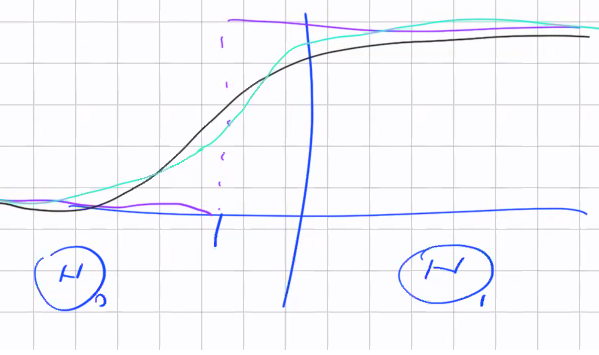
\includegraphics[scale=0.7]{images/Stat_Theory_Lecture_!3.png}
\end{center}
\begin{definition}
A uniformly most powerful test with significance $\alpha$ is a test that satisfies
\begin{itemize}
    \item \[\sup_{\theta\in\Theta_0}\pi(\theta)=\alpha\]
    \item Assume that $\pi_1(\theta)$ is a power function for a different test with significance $\alpha$, we have that for all $\theta$
    \[\pi(\theta)\geq\pi_1(\theta)\]
\end{itemize}
\end{definition}
\newpage
\begin{definition}
For a family of distributions $F_{\theta}$ where $\Theta$ is one-dimensional. This family has monotone likelihood ratios if there is a statistic $T(\overrightarrow{Y})$ such that for all $\theta_1<\theta_2$ we have that
\[\frac{f_{\theta_0}(\overrightarrow{y})}{f_{\theta_1}(\overrightarrow{y})}\]
is a monotone non-decreasing function of $T(\overrightarrow{Y})$. 
\end{definition}
\begin{claim}
Assume $\overrightarrow{Y}\sim f_{\theta}(\overrightarrow{y})$ where $f_{\theta}\in F_{\theta}$ from a family of monotone likelihood ratios with statistic $T(\overrightarrow{Y})$ Then there is a uniformly most powerful test with significance $\alpha$ for the hypothesis 
\[H_1:\theta>\theta_0\]
where the test is
\[T(\overrightarrow{Y})\geq C\]
And
\[\alpha = \mathbb{P}_{\theta_0}(T(\overrightarrow{Y})\geq C)\]
\end{claim}
\begin{proof}
Assume first that $\theta_1>\theta_0$. We will create a test with maximal power for the hypothesis 
\[H_0:\theta=\theta_0\text{, } H_1:\theta=\theta_1\]
Using Neyman-Pearson the maximal power test is the LRT. Meaning
\[\lambda(\overrightarrow{y})=\frac{f_{\theta_1}(\overrightarrow{y})}{f_{\theta_0}(\overrightarrow{y})}>C\]
Where C is determined such that
\[\mathbb{P}_{\theta_0}(\lambda(\overrightarrow{y}>C))  =\alpha\]
This is independent of $\theta_1$ and so this is the maximal power test for $\theta_1\in\Theta_1$.
Now assume that $\Theta_0:=(-\infty, \theta_0]$. It suffices to show that
\[\text{For every }\theta\in\Theta_0 we have that \mathbb{P}_{\theta}(\overrightarrow{y}\in\Omega_1)\leq\alpha \]
Take $\theta_2<\theta_0$ and build the following test that distinguishes between the following hypotheses:
\[H_0:\theta=\theta_2\text{, }H_1:\theta=\theta_0\]
From Neyman-Pearson we know that the LRT is the maximal power test
\[\lambda(\overrightarrow{y})\geq C'\]
where 
\[\mathbb{P}_{\theta_2}(T(\overrightarrow{y})\geq C) = \alpha'\]
and
\[\pi = \mathbb{P}_{\theta_0}(T(\overrightarrow{Y})\geq C) = \alpha\]
We want to show that $\alpha\geq\alpha'$. We will build another test - flip a biased coin with probability $\alpha'$ for heads and declare $H_1$, otherwise maintain null hypothesis . It can be easily seen that the power and significance $\alpha'$ and so $\alpha'\leq\alpha$ and we are done. (Notice that this means appending a sampling of a bernoulli variable to the sampling)
\end{proof}
\subsection{Generalized Likelihood Ratio Test}
Given composite hypotheses we can redefine the likelihood ratio
\[\lambda=\frac{\sup_{\theta\in\Theta} f_{\theta}(\overrightarrow{y})}{\sup_{\theta\in\Theta_0} f_{\theta}(\overrightarrow{y})}\]
This is called the general likelihood ratio. 
\begin{definition}
A GLRT is a test for composite hypothesis where the test is
\[\lambda(\overrightarrow{y})\geq C\]
\end{definition}
Notice that both the denominator and the numerator are MLE's for different coefficient spaces. Usually in order to find a good way to express this is using some statistic $T(\overrightarrow{Y})$ to help us inverse the $\lambda$ function. 
\begin{example}
Sample $Y_1,\dots,Y_n\sim\mathcal{N}(\mu,\sigma^2)$, with unknown $\sigma^2$. Now consider 2 hypotheses
\[H_0:\mu=\mu_0\text{, } H_1:\mu\neq\mu_0\]. 
MLE we have already seen for the normal distribution. This is
\[\left(\bar{Y}, \frac{1}{n}\sum_{i=1}^n \left(y_i - \bar{Y}\right)^2\right)\]
MLE estimate for $H_0$ is 
\[\hat{\mu_0}=\mu_0, \hat{\sigma^2_0} = \frac{1}{n}\sum_{i=1}^n \left(y_i-\mu\right)^2\]
The likelihood in general is 
\[L(\hat{\mu},\hat{\sigma^2}; \overrightarrow{y})=\left(\frac{1}{\sigma\sqrt{2\pi}}\right)^ne^{-\frac{1}{2} \sum_{i=1}^n (\frac{y_i-\bar{y}}{\hat{\sigma}})^2}\]
Looking at the ratio between this and \[L(\hat{\mu_0},\hat{\sigma_0^2}; y)\]
We have 
\[\left(1+\frac{1}{n-1}\left(\frac{\bar{y}-\mu_0}{s/\sqrt{n}}\right)^2\right)^{\frac{1}{2} n}\]
Where \[s^2:= \frac{1}{n-1}\sum_{i=1}^n (y_i-\mu_0)^2\]
Now take statistic
\[T(\overrightarrow{Y}) = \frac{\bar{y}-\mu_0}{S/\sqrt{n}}\]
Therefore the test will look like
\[|T(\overrightarrow{Y})|\geq C \text{ where } \mathbb{P}_{\mu_0}(|T(\overrightarrow{Y})\geq C|) = \alpha\]
\end{example}
For composite hypotheses we enter a supremum in the following sense
\[\text{p-value}:=\sup_{\theta\in\Theta_0}\mathbb{P}_{\theta}\left(T(\overrightarrow{Y})>T(\overrightarrow{y})\right)\]
\subsection{Connection Between hypothesis testing to the significance interval}
A significance interval with significance $1-\alpha$ for $\theta$ is the interval $\left(L(\overrightarrow{y}), U(\overrightarrow{y})\right)$
Such that 
\[\mathbb{P}_{\theta}(L\leq\theta\leq U)\geq1-\alpha\]
If we define $H_0:\theta=\theta_0$. We will define the test where we find the significance interval. If $\theta_0\in(L,U)$ then $H_0$ otherwise $H_1$. This is a test with significance $\alpha$. (This is a pretty simple observation).
\\\\\\\\\\
And we are done
\end{document}
